
\chapter{Resultados} \label{chapter6}

Este Capítulo apresenta os resultados obtidos por meio de consultas SQL e do processo de mineração de dados, seguindo a metodologia apresentada no Capítulo \ref{chapter5}. A Seção \ref{sec61} apresenta os resultados observados para os alunos por meio de consultas ao banco de dados, e a Seção \ref{sec62} apresenta os resultados obtidos para a evasão por meio do processo de mineração de dados realizado no Weka.

\section{Resultados Obtidos por Consultas SQL ao Banco de Dados} \label{sec61}

Os gráficos e resultados apresentados nesta Seção foram elaborados tomando por base consultas SQL realizadas no banco de dados. Foram selecionados os alunos para os quais foram verificados registros acadêmicos na tabela \textit{Histórico} a partir do primeiro semestre de curso, entre o ano de 2000 e 2013, o que indica que o aluno comprovadamente cursou uma ou mais das disciplinas analisadas durante os três primeiros semestres de curso. Ao todo, foram contabilizados 1.105 registros.

\subsection{Visão Geral} \label{visao_geral}
Dos 1.105 alunos identificados na base de dados que ingressaram no curso de Ciência da Computação da Universidade de Brasília entre 2000 e 2013, foram identificados 33,6\% dos alunos como formados, 36,9\% como desligados e 29,5\%  como cursando em 2014, conforme a Figura \ref{grafico9}. Ao verificar os percentuais obtidos por análise estatística dos dados, percebe-se que o índice de formatura entre o ano de 2000 e 2013 é menor se comparado ao índice de desligamento.

\begin{figure}[!h]
	\centering
	{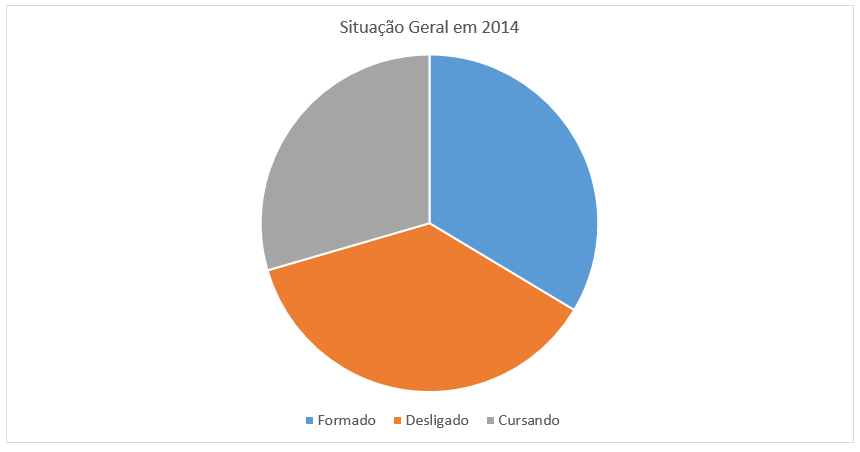
\includegraphics[width=14cm, height=7cm]{images/grafico9}}
	\caption {Situação dos alunos ingressantes entre 2000 e 2013 no ano de 2014.}
	\label{grafico9}
\end{figure}
  
Pela Figura \ref{grafico1}, a linha de tendência gerada pelo Excel aponta para o crescimento da quantidade de alunos ingressantes no curso de Ciência da Computação para os próximos semestres a partir de 2013. Entre o ano de 2000 e 2013, o número de alunos ingressantes variou entre 30 e 52 alunos por semestre.

\begin{figure}[!h]
	\centering
	{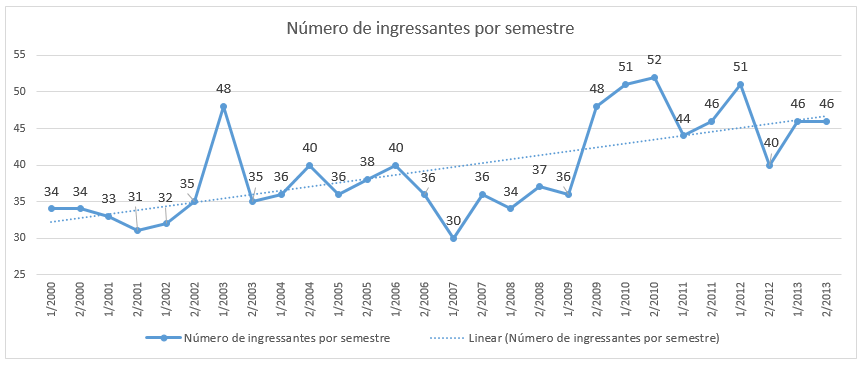
\includegraphics[width=16cm, height=6cm]{images/grafico1}}
	\caption {Gráfico de Ingressantes por Semestre no curso de Ciência da Computação da Universidade de Brasília entre o ano de 2000 e 2013.}
	\label{grafico1}
\end{figure}
  

A Figura \ref{grafico2} mostra o quantitativo de ingressantes, formados e desligados por semestre entre o ano de 2000 e 2013. O gráfico representa a situação dos alunos ingressantes por semestre no ano de 2014, período no qual os dados analisados foram obtidos. Tomando como exemplo os alunos que ingressaram no primeiro semestre de 2004, em 2014 não havia alunos na situação de cursando, 15 alunos foram constatados como desligados e 25 formados. Considerando que o aluno conclua o curso, em média, entre 10 e 12 semestres, justifica-se o crescimento da quantidade de alunos cursando e o decrescimento da quantidade de alunos formados a partir do ano de 2008. Anterior ao ano de 2008, o primeiro semestre de 2003 apresentou a maior quantidade de alunos que concluíram a graduação, somando 28 alunos formados. Se comparada a quantidade de formados pela quantidade de ingressantes por semestre, o segundo semestre de 2001 apresentou o melhor aproveitamento de alunos, com 80,6\% dos alunos de formados. Em contrapartida, o primeiro semestre de 2004 e o primeiro semestre de 2006 apresentaram a maior quantidade de alunos que não concluíram a graduação, somando 22 alunos desligados cada. Se comparada a quantidade de desligados pela quantidade de alunos ingressantes por semestre, o primeiro semestre de 2004 apresentou o pior aproveitamento de alunos, pois 61,1\% dos alunos ingressos saíram do curso antes do término. Cada coluna no gráfico representa a quantidade de alunos que foram identificados como cursando, formados ou desligados no ano de 2014.


\begin{figure}[!h]
	\centering
	{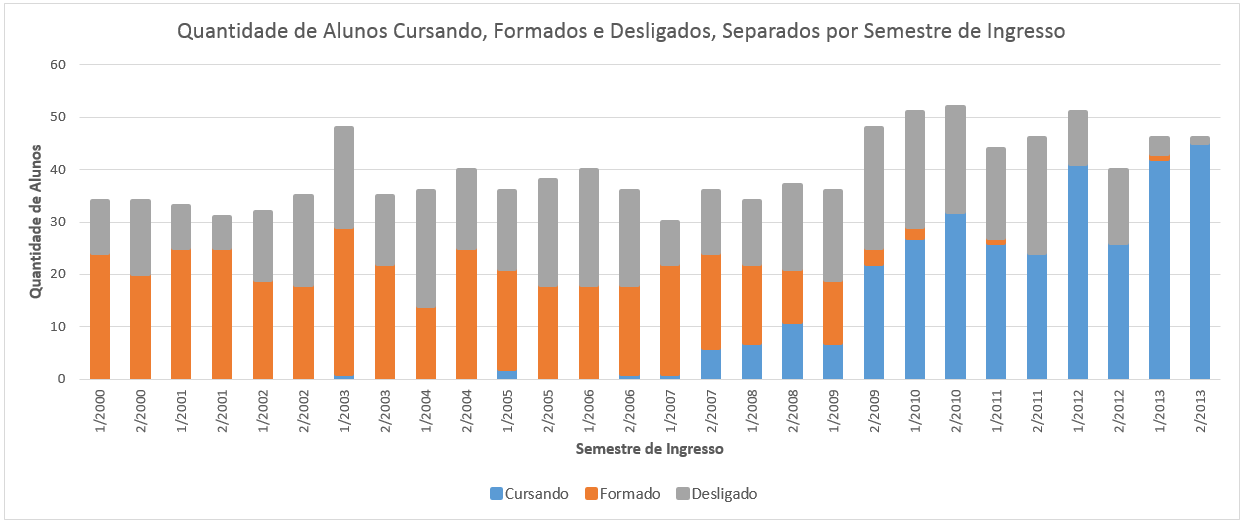
\includegraphics[width=16cm, height=5cm]{images/grafico2}}
	\caption {Situação dos alunos ingressantes por semestre no curso de Ciência da Computação da Universidade de Brasília no ano de 2014.}
	\label{grafico2}
\end{figure}


A Figura \ref{grafico10} apresenta as formas de ingresso para os alunos ingressantes entre 2000 e 2013, dada a situação do aluno em 2014. Dentre os alunos formados, 68,2\% ingressaram pelo vestibular, 26,1\% pelo Programa de Avaliação Seriada, 5,1\% por transferência obrigatória  e 0,6\% ingressaram por acordo cultural.

\begin{figure}[!htb]
	\centering
	{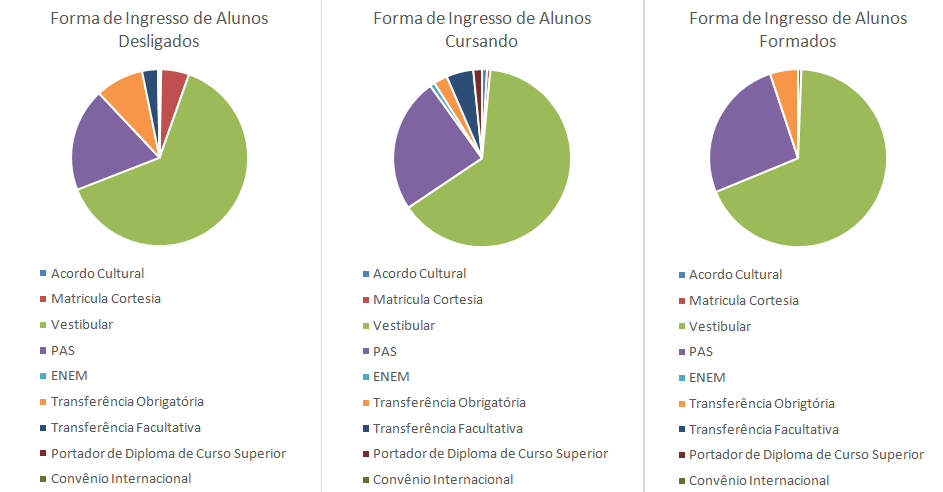
\includegraphics[width=14cm, height=7cm]{images/grafico10}}
	\caption {Formas de ingresso para os alunos identificados como formados, desligados e cursando em 2014.}
	\label{grafico10}
\end{figure}

Entre os alunos identificados como cursando, 64,1\% ingressaram pelo vestibular, 24,5\% pelo PAS, 4,9\% por transferência facultativa, 2,5\% por transferência obrigatória, 1,6\% por ser portador de diploma de curso superior e 0,9\% pelo Exame Nacional do Ensino Médio (ENEM).

Dentre os alunos identificados como desligados, 63,7\% ingressaram pelo vestibular, 18,9\% pelo PAS, 8,8\% por transferência obrigatória, 5,1\% por matricula cortesia, 2,9\% por transferência facultativa, 0,3\% por convênio internacional e 0,3\% por acordo cultural. Do gráfico, percebe-se que entre 2000 e 2013 não houve registros de formados por alunos ingressos por matrícula cortesia, ENEM, transferência facultativa, por ser portador de diploma de curso superior e convênio internacional.
 
 Analisando os motivos de evasão por semestre, percebe-se que os motivos mais recorrentes para justificar a evasão dos alunos em geral foram o desligamento por abandono, por não cumprimento de condição, desligamento voluntário, desligamento por reprovar três vezes a mesma disciplina obrigatória, por novo vestibular e por transferência. Do mesmo modo, pode-se constatar que o desligamento por falecimento e por decisão judicial são eventuais, ocorrendo em menor frequência ao longo dos anos. Dos alunos desligados entre 2000 e 2013, apenas 0,2\% foram desligados por falecimento e 0,7\% por decisão judicial. A Tabela \ref{desligamento_geral} detalha o percentual de alunos ingressantes por semestre, entre o ano de 2000 e 2013, que foram identificados como desligados em 2014, separados por motivo de desligamento. Foram considerados para a tabela apenas os motivos mais recorrentes de desligamento identificados na base de dados.
 
 \begin{longtable}{C{1,8cm}|C{1,9cm}C{2,0cm}C{1,9cm}C{2,1cm}C{2cm}C{2,0cm}}
 	\caption{Percentual de alunos desligados por motivo.} 	\label{desligamento_geral} \\
 	\hline
 	Semestre & \multicolumn{6}{|c}{Percentual (\%) de Desligamento por Motivo}\\ 
 	\hline
 	& Abandono & Não Cumpriu Condição & Voluntário & Reprovou 3 vezes Mesma Disciplina Obr. & Novo Vestibular & Transferência\\
 	\hline
 	1/2000 & 10 & 60 & 30 & 0 & 0 & 0\\
 	2/2000 & 28,6 & 50 & 14,3 & 0 & 0 & 7,1\\
 	1/2001 & 12,5 & 75 & 12,5 & 0 & 0 & 0\\
 	2/2001 & 33,3 & 16,7 & 50 & 0 & 0 & 0\\
 	1/2002 & 0 & 46,1 &  38,5 & 0 & 7,7 & 7,7\\
 	2/2002 & 0 & 46,1 & 38,5 & 0 & 7,7 & 7,7\\
 	1/2003 & 21,05 & 47,4 & 10,5 & 21,05 & 0 & 0\\
 	2/2003 & 23 & 38,5 & 15,4 & 7,7 & 7,7 & 7,7\\
 	1/2004 & 27,3 & 27,3 & 36,4 & 0 & 0 & 4,5\\
 	2/2004 & 6,7 & 46,7 & 26,7 & 0 & 0 & 0\\
 	1/2005 & 40 & 26,7 & 20 & 13,3 & 0 & 0\\
 	2/2005 & 20 & 60 & 5 & 0 & 10 & 5\\
 	1/2006 & 18,2 & 45,5 & 4,6 & 0 & 9 & 22,7\\
 	2/2006 & 11,1 & 38,9 & 27,8 & 11,1 & 11,1 & 0\\
 	1/2007 & 12,5 & 37,5 & 37,5 & 0 & 0 & 12,5\\
 	2/2007 & 33,3 & 58,3 & 0 & 8,4 & 0 & 0\\
 	1/2008 & 8,3 & 41,7 & 17,7 & 0 & 33,3 & 0\\
 	2/2008 & 6,25 & 37,5 & 25 & 25 & 0 & 6,25\\
 	1/2009 & 5,9 & 23,5 & 29,4 & 17,6 & 23,5 & 0\\
 	2/2009 & 4,35 & 26,1 & 8,7 & 17,4 & 39,1 & 4,35\\
 	1/2010 & 13,6 & 36,4 & 4,6 & 0 & 31,8 & 13,6\\
 	2/2010 & 15 & 55 & 0 & 10 & 20 & 0\\
 	1/2011 & 5,9 & 52,9 & 5,9 & 35,3 & 0 & 0\\
 	2/2011 & 0 & 77,3 & 0 & 9,1 & 9,1 & 4,5\\
 	1/2012 & 10 & 70 & 0 & 0 & 20 & 0\\
 	2/2012 & 0 & 78,6 & 0 & 7,1 & 14,3 & 0\\
 	1/2013 & 0 & 33,3 & 33,3 & 0 & 33,3 & 0\\
 	\hline
 \end{longtable} 

\subsection{Análise dos Alunos por Gênero} \label{analise_genero}

A Figura \ref{grafico3} mostra a quantidade de alunas ingressantes por semestre entre 2000 e 2013, e a quantidade das mesmas que foram identificadas como formadas no ano de 2014. Pelo gráfico, o primeiro semestre de 2005 e o primeiro semestre de 2010 registraram a maior quantidade de alunas ingressantes, totalizando 10 alunas cada. Se comparada a quantidade de alunas formadas sobre o total de alunas ingressantes por semestre, o primeiro semestre de 2001 apresentou o melhor aproveitamento das alunas, pois 100\% das alunas ingressantes formaram-se, seguido do primeiro semestre de 2003, com aproveitamento de 86\% de alunas formadas. 
  
\begin{figure}[!h]
	\centering
	{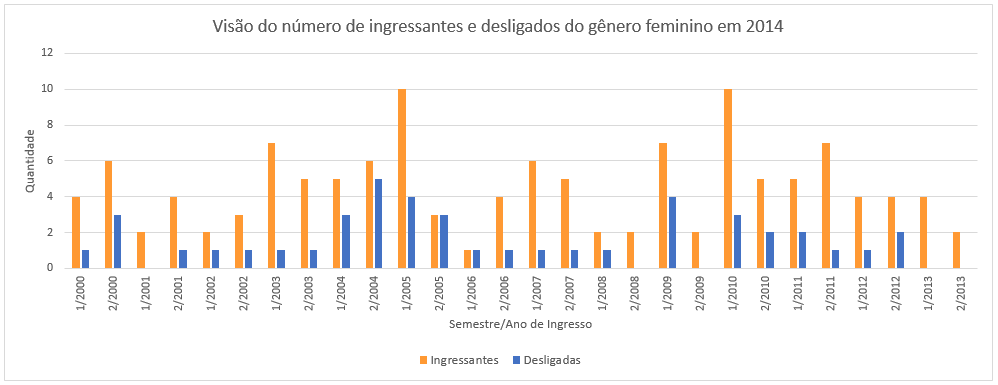
\includegraphics[width=16cm, height=6cm]{images/grafico3}}
	\caption {Quantidade de alunas ingressantes por semestre  entre o ano de 2000 e 2013 e quantidade de alunas que foram identificadas como formadas no curso de Ciência da Computação da Universidade de Brasília no ano de 2014.}
	\label{grafico3}
\end{figure}

A Figura \ref{grafico4} mostra a quantidade de alunos do sexo masculino ingressantes por semestre entre 2000 e 2013, e a quantidade dos mesmos que foram identificados como formados no ano de 2014. Ao comparar o número de alunos ingressantes e formados por gênero, percebe-se que há uma predominância dos alunos do sexo masculino no curso de Ciência da Computação da Universidade de Brasília. Se comparada a quantidade de alunos formados sobre o total de alunos ingressantes do sexo masculino, o segundo semestre de 2001 e o primeiro semestre de 2001 apresentaram o melhor aproveitamento de alunos, pois formaram 81\% e 74\% dos alunos ingressantes, respectivamente. 

\begin{figure}[!h]
	\centering
	{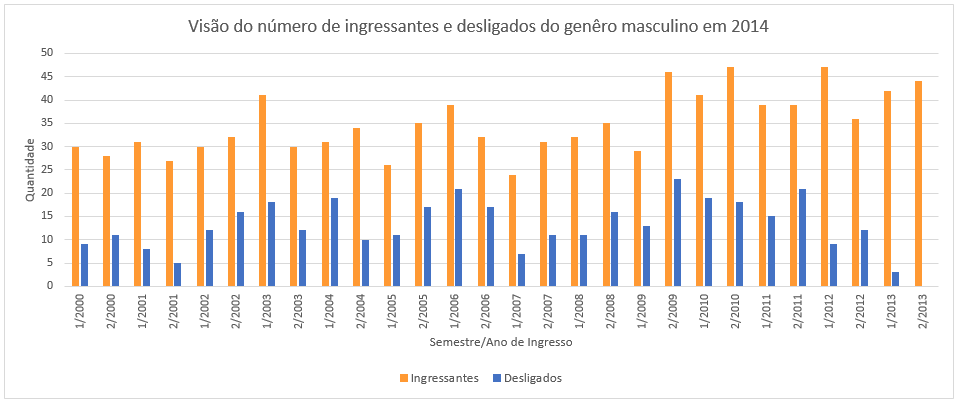
\includegraphics[width=16cm, height=6cm]{images/grafico4}}
	\caption {Quantidade de alunos do sexo masculino ingressantes por semestre  entre o ano de 2000 e 2013 e quantidade de alunos que foram identificados como formados no curso de Ciência da Computação da Universidade de Brasília no ano de 2014.}
	\label{grafico4}
\end{figure}

A Figura \ref{grafico7} apresenta a visão do percentual de desligamento geral em 2014, separado por semestre. Do total de alunos que ingressaram no primeiro semestre de 2004 e no primeiro semestre de 2006, 61,1\% e 55\%, respectivamente, foram identificados como desligados em 2014, sendo estes considerados os semestres com maior percentual de evasão entre 2000 e 2013.

\begin{figure}[!h]
	\centering
	{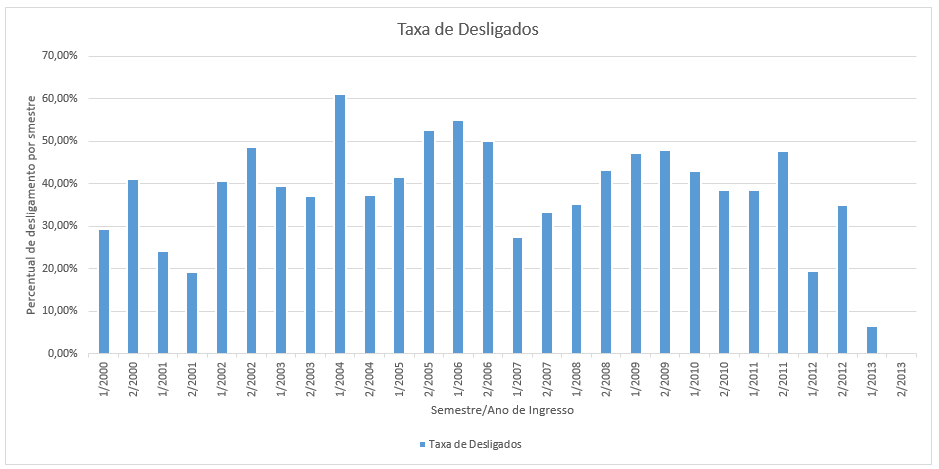
\includegraphics[width=16cm, height=6cm]{images/grafico7}}
	\caption {Visão da taxa de desligamento geral por semestre no ano de 2014.}
	\label{grafico7}
\end{figure}


As Figuras \ref{grafico5} e \ref{grafico6} mostram o comparativo de alunos que foram identificados como formados e desligados no ano de 2014, separados por gênero. Entre 2000 e 2008, percebe-se a maior variação da taxa de alunos formados e desligados para o gênero feminino, tendo sido constatados semestres com 100\% de aproveitamento (primeiro semestre de 2001) e com 0\% de aproveitamento (segundo semestre de 2005 e primeiro semestre de 2006) das alunas ingressantes. Para o gênero masculino, a taxa de formados por semestre variou entre 38,1\% (primeiro semestre de 2004) e 81,5\% (segundo semestre de 2001). 

\begin{figure}[!h]
	\centering
	{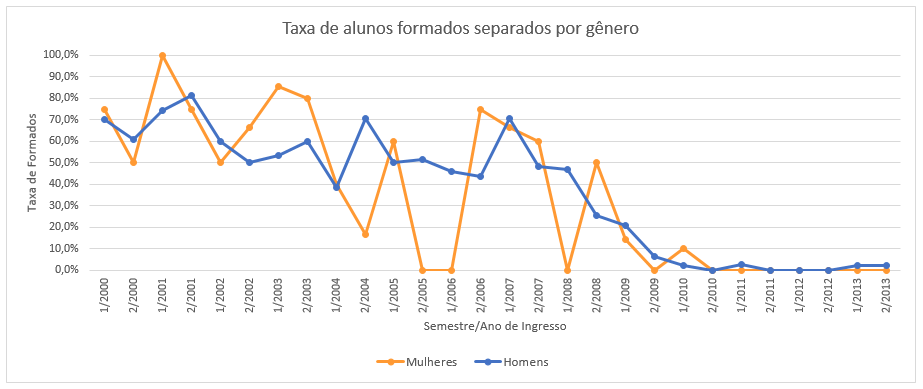
\includegraphics[width=16cm, height=6cm]{images/grafico5}}
	\caption {Taxa de alunos formados por semestre entre o ano de 2000 e 2013 separados por gênero.}
	\label{grafico5}
\end{figure}

\begin{figure}[!h]
	\centering
	{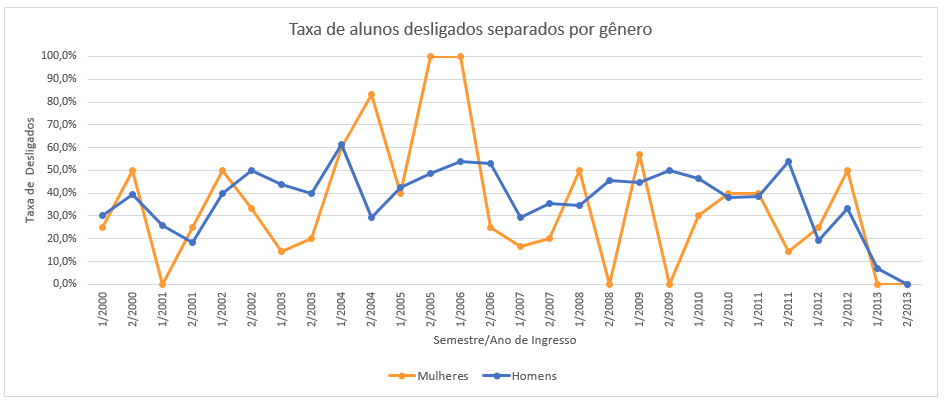
\includegraphics[width=16cm, height=6cm]{images/grafico6}}
	\caption {Taxa de alunos desligados por semestre entre o ano de 2000 e 2013 separados por gênero.}
	\label{grafico6}
\end{figure}


A Figura \ref{grafico8} apresenta as formas de saída observadas para os alunos que foram identificados como desligados em 2014. Dos alunos ingressantes entre 2000 e 2013, 46,6\% foram desligados por não cumprimento de condição, 14,2\% por abandono, 14,2\% por desligamento voluntário, 11,8\% por novo vestibular, 10,3\% por reprovar três vezes a mesma disciplina obrigatória, 2\% por transferência, 0,7\% por decisão judicial e 0,2\% por falecimento.

\begin{figure}[!h]
	\centering
	{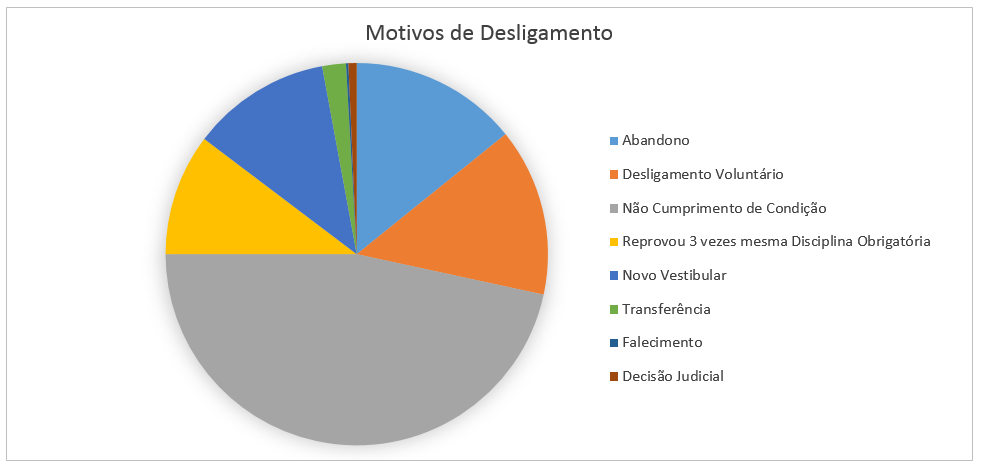
\includegraphics[width=13cm, height=6cm]{images/grafico8}}
	\caption {Formas de desligamento identificadas para os alunos em geral ingressos entre 2000 e 2013.}
	\label{grafico8}
\end{figure}
 

A partir dos dados gerais obtidos entre 2000 e 2013 e analisando-os por gênero dos alunos, pode-se constatar que:
\begin{itemize}
	\item Entre o ano de 2000 e 2013, foram contabilizadas 127 alunas que matricularam-se no curso de Ciência da Computação. Deste total, no ano de 2014 haviam 34,7\% alunas desligadas, 36,2\% formadas e  29,1\% cursando. No mesmo período, foram contabilizados 978 alunos do sexo masculino no curso de Ciência da Computação. Deste total, no ano de 2014, haviam 37,2\% alunos desligados, 33,3\% formados e 29,5\% cursando;
	
	\item Dentre as alunas formadas, 76\% não informaram a escola de origem onde cursaram o Ensino Médio. Em relação aos alunos formados, esse percentual aumenta para 78,5\%;
	
	\item 97,1\% das alunas formadas ingressaram na UnB pelo sistema universal e 2,9\% pelo sistema de cotas para negros.  Dos alunos formados, 95,1\% ingressaram pelo sistema universal e 4,9\% por sistemas de cotas para negros;
	
	\item Das alunas formadas que informaram a escola de origem onde concluíram o Ensino Médio, 90,9\% são oriundas de escola particular e 9,1\% de escola pública.  Dentre os alunos formados que informaram a escola de origem, 84,3\% cursaram o Ensino Médio em escola particular e 25,7\% em escola pública;
	
	\item Das alunas formadas que cursaram o Ensino Médio em escola particular, 80\% foram aprovadas pelo sistema universal e 20\% pelo sistema de cotas para negros. Entre as alunas formadas que cursaram o Ensino Médio em escola pública, 100\% foram aprovadas pelo sistema universal. Para os alunos formados que cursaram o Ensino Médio em escola particular, 93,2\% foram aprovados pelo sistema universal e 6,8\% pelo sistema de cotas para negros. Entre os alunos formados que cursaram o Ensino Médio em escola pública, 91\% foram aprovados pelo sistema universal e 9\% pelo sistema de cotas para negros;
	
	\item As alunas formadas ingressaram no curso na faixa etária dos 16 aos 32 anos, sendo que 76\% ingressou no curso com idade entre 17 e 19 anos.  Os alunos formados ingressaram no curso na faixa etária dos 16 a 35 anos, e destes, 73,5\% ingressaram com idade entre 17 e 19;
	
	\item Das alunas formadas, 60,9\% ingressaram pelo vestibular, 26\% pelo Programa de Avaliação Seriada (PAS), 10,9\% por transferência obrigatória e 2,2\% por acordo cultural;
	
	\item Dos alunos formados, 29,8\% formaram-se antes do 10º semestre, 55,1\% entre o 10º e 12º semestre, e 15,1\% após o 12º semestre; 
	
	\item As alunas formadas levaram em média 11 semestres para concluir o curso, e os alunos em média 10 semestres;
	
	\item As alunas desligadas cursaram, em média, 5 semestres. Para os alunos desligados, a média aumenta para 6 semestres;
	
	\item Das alunas desligadas, 68\% ingressaram na faixa etária entre 17 e 19 anos;
	
	\item 70\% das alunas desligadas não informaram em qual tipo de escola (pública ou particular) cursaram o Ensino Médio. Para os alunos, esse percentual é reduzido para 64,3\%;
	
	\item Das alunas desligadas que informaram a escola de origem na qual cursaram o Ensino Médio, 84\% são oriundas de escola particular, e entre os alunos, 70,8\% são oriundos de escola particular;
	
	\item Todas as alunas desligadas que cursaram o Ensino Médio em escola pública ou particular foram aprovadas pelo sistema universal. Dos alunos desligados que cursaram o Ensino Médio em escola particular, 87\% foram aprovados pelo sistema universal e  13\% pelo sistema de cotas para negros. Dos alunos desligados que cursaram o Ensino Médio em escola pública, 5,3\% foram aprovados pelo sistema de cotas para escola pública de alta renda PPI, 28,9\% pelo sistema de cotas para negros e 65,8\% pelo sistema universal; 
	
	\item 97,7\% das alunas desligadas foram aprovadas pelo sistema universal e 2,3\% pelo sistema de cotas para negros. Dos alunos desligados, 87,4\% foram aprovados pelo sistema universal, 12,1\% pelo sistema de cotas para negros e 0,5\% por cotas para escola pública de alta renda PPI;
	
	\item Entre as alunas desligadas, 47,7\% ingressaram pelo vestibular, 22,5\% pelo Programa de Avaliação Seriada (PAS), 15,9\% por transferência obrigatória e 13,6\% por matrícula cortesia. Entre os alunos desligados, 0,3\% ingressaram por acordo cultural, 0,3\% por convênio internacional, 4,1\% por matrícula cortesia, 18,4\% pelo Programa de Avaliação Seriada (PAS), 3,3\% por transferência facultativa, 8\% por transferência obrigatória e 65,6\% pelo vestibular;
	
	
	\item Dos alunos desligados que cursaram o Ensino Médio em escola particular, 87\% foram aprovados pelo sistema universal e  13\% pelo sistema de cotas para negros. Dos alunos desligados que cursaram o Ensino Médio em escola pública, 5,3\% foram aprovados pelo sistema de cotas para escola pública de alta renda PPI, 28,9\% pelo sistema de cotas para negros e 65,8\% pelo sistema universal; 
	
	\item Entre todas as alunas desligadas, 22,7\% foi por abandono, 6,8\% por decisão judicial, 22,7\% por não cumprimento de condição, 25\% por desligamento voluntário, 18,2\% por novo vestibular, 2,3\% por reprovar três vezes a mesma disciplina obrigatória e 2,3\% por transferência. 	Entre todos os alunos desligados, 13,2\% foi por abandono, 49,4\% por não cumprimento de condição, 12,9\% por desligamento voluntário, 0,3\% por falecimento, 11\% por novo vestibular, 11,3\% por reprovar três vezes a mesma disciplina obrigatória e 1,9\% por transferência;
	
	\item 56,8\% das alunas desligadas saíram do curso entre o 1º e o 3º semestre, 18,2\% saíram entre o 4º e o 7º semestre e 25\% saíram após o 7º semestre do curso. Analisando o mesmo cenário para os alunos desligados, 36\% saíram entre o 1º e o 3º semestre, 41,2\% entre o 4º e o 7º semestre e 22,8\% após o 7º semestre;
	
	\item Das alunas desligadas entre o 1º e o 3º semestre do curso, 12\% foi por abandono, 12\% por decisão judicial, 28\% por desligamento voluntário, 20\% por não cumprimento de condição, 24\% por novo vestibular e 4\% por transferência. Dos alunos desligados no mesmo período, 6,1\% saíram por motivo de abandono,  53,4\% por não cumprimento de condição, 16,8\% por desligamento voluntário, 9,2\% por novo vestibular, 11,4\% por reprovar três vezes a mesma disciplina obrigatória e 3\% por transferência;
	
	\item Das alunas desligadas entre o 4º e o 7º semestre do curso, 12,5\% foi por abandono, 37,5\% por não cumprimento de condição, 25\% por desligamento voluntário, 12,5\% por novo vestibular e 12,5\% por reprovar três vezes a mesma disciplina obrigatória.  Dos alunos desligados no mesmo período, 12,8\% saíram por motivo de abandono, 50\% por não cumprimento de condição, 11,3\% por desligamento voluntário, 15,3\% por novo vestibular, 9,3\% por reprovar três vezes a mesma disciplina obrigatória e 1,3\% por transferência; 
	
	\item Das alunas desligadas após o 7º semestre do curso, 54,5\% foi por motivo de abandono, 18,2\%  por não cumprimento de condição, 18,2\% por desligamento voluntário e 0,1\% por novo vestibular. Dos alunos desligados após o 7º semestre, 25,3\% saíram por motivo de abandono, 42,2\% por não cumprimento de condição, 9,6\% por desligamento voluntário, 1,2\% por falecimento, 6\% por novo vestibular, 14,5\% por reprovar três vezes a mesma disciplina obrigatória e 1,2\% por transferência.
\end{itemize}

\subsection{Análise das Disciplinas}

A partir da análise dos dados armazenados nas tabelas \textit{evasao\_cic, evasao\_mat} e \textit{evasao\_cic}, constatou-se que:
\begin{itemize} 
	\item Dos alunos em geral que cursaram a disciplina Computação Básica, 17,35\% não cursaram a disciplina Estruturas de Dados e 31,85\% não cursaram a disciplina Programação Sistemática. Considerando apenas os alunos desligados que cursaram a disciplina Computação Básica, 31,12\% não cursaram a disciplina Estruturas de Dados e 55,63\% não cursaram a disciplina Programação Sistemática;
	\item Dos alunos em geral que cursaram a disciplina Cálculo 1, 25,21\% não cursaram a disciplina Cálculo 2 e 38,65\% não cursaram a disciplina Cálculo 3. Considerando apenas os alunos desligados que cursaram a disciplina Cálculo 1, 36,31\% não cursaram a disciplina Cálculo 2 e 60,83\% não cursaram a disciplina Cálculo 3;
	\item Dos alunos em geral que cursaram a disciplina Física 1, 28,90\% não cursaram a disciplina Física 2 e 42,18\% não cursaram a disciplina Física 3. Considerando apenas os alunos desligados que cursaram a disciplina Física 1, 48,71\% não cursaram a disciplina Física 2 e 68,46\% não cursaram a disciplina Física 3.
\end{itemize}

A Figura \ref{taxa_reprovados} mostra a taxa de reprovação geral entre 2000 e 2013 para as disciplinas ofertadas nos três primeiros semestres do curso . Analisando as taxas de reprovação por departamento, as disciplinas observadas com maiores índices de reprovação foram Computação Básica (26,06\%), Cálculo 3 (45,2\%) e Física 1 (37,13\%). Analisando todas as disciplinas apresentadas no gráfico, a disciplina Cálculo 3 apresenta a maior taxa de reprovação, seguida de Cálculo 1 (38,09\%) e Física 1 (37,13\%).

\begin{figure}[!h]
	\centering
	{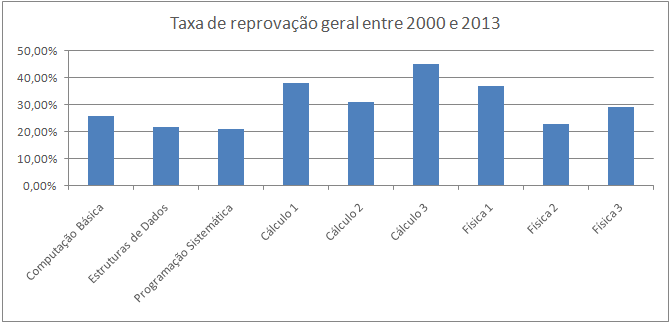
\includegraphics[width=13cm, height=6cm]{images/taxa_reprovados}}
	\caption {Taxa de reprovação geral entre 2000 e 2013 para as disciplinas obrigatórias ofertadas nos três primeiros semestres.}
	\label{taxa_reprovados}
\end{figure}

Ao analisar a taxa de desligamento por disciplina considerando apenas os dados dos alunos identificados como desligados, constatou-se que o índice de reprovação é superior se comparado aos índices de reprovação geral, conforme mostrado na Figura \ref{reprovados_desligados}. Para todas as disciplinas analisadas, com exceção da disciplina Estruturas de Dados, foram verificadas taxas de reprovação acima de 50\%. Analisando por departamento, as disciplinas observadas com maiores índices de reprovação para os alunos desligados foram Programação Sistemática (53,59\%), Cálculo 3 (80,69\%) e Física 3 (73,17\%). Analisando todas as disciplinas apresentadas no gráfico, a disciplina Cálculo 3 apresentou a maior taxa de reprovação, seguida de Física 3 e Cálculo 1 (70,84\%).

\begin{figure}[!h]
	\centering
	{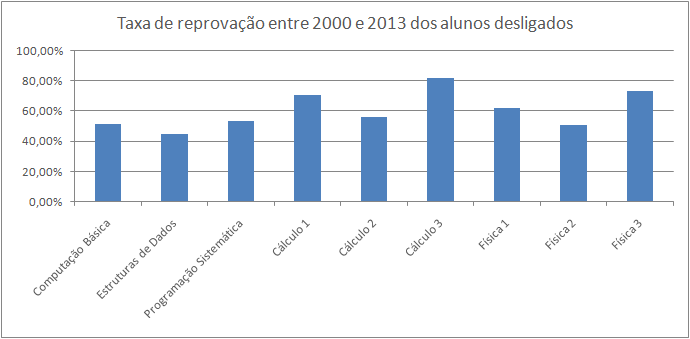
\includegraphics[width=13cm, height=6cm]{images/reprovados_desligados}}
	\caption {Taxa de reprovação entre 2000 e 2013 dos alunos desligados para as disciplinas obrigatórias ofertadas nos três primeiros semestres.}
	\label{reprovados_desligados}
\end{figure}

A Figura \ref{reprova3} apresenta o percentual geral de alunos que reprovaram três vezes a mesma disciplina para os três primeiros semestres. Para a disciplina Programação Sistemática, não foram identificados alunos que reprovaram ao cursar pela terceira vez. Para as demais disciplinas, foi identificada uma variação entre 0,76\% (Cálculo 3) e 3,64\% (Física 1). Analisando por departamento, as disciplinas observadas com maiores índices de reprovação ao serem cursadas pela terceira vez foram Computação Básica (2,44\%), Cálculo 1 (2,05\%) e Física 1 (3,64\%).

\begin{figure}[!h]
	\centering
	{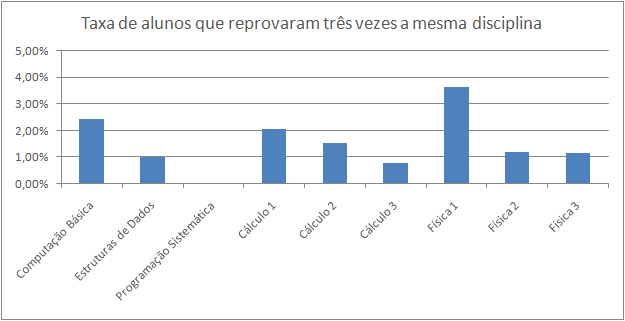
\includegraphics[width=13cm, height=6cm]{images/reprova3}}
	\caption {Percentual de alunos que reprovaram três vezes a mesma disciplina obrigatória.}
	\label{reprova3}
\end{figure}

As Tabelas \ref{mencao_geral} e \ref{mencao_desligados} apresentam, respectivamente, o percentual de menções obtidas pelos alunos em geral e pelos alunos desligados nas disciplinas obrigatórias dos três primeiros semestres. Foram consideradas para o cálculo dos percentuais apenas as primeiras menções obtidas pelos alunos ao cursaram as disciplinas. 

Das menções obtidas pelos alunos em geral, foi identificado que nas disciplinas ofertadas pelo Departamento de Matemática (MAT-UnB), o percentual de menções SR, II e MI é maior se comparadas as demais disciplinas apresentadas. Para as disciplinas ofertadas pelo Instituto de Física (IF-UnB), foi verificado um maior percentual de menções MM, e para o Departamento de Ciência da Computação foi verificado um maior percentual de menções MS e SS nas disciplinas introdutórias. 

Para todas as disciplinas apresentadas na Tabela \ref{mencao_geral}, as menções TR e TJ varia entre 0\% e 6,1\%. Analisando os maiores percentuais por menção, verifica-se que:
\begin{itemize}
	\item O maior percentual de menção TR foi verificado em Cálculo 3, com 6,1\%;
	\item O maior percentual de menção TJ foi verificado em Física 1, com 1\%;
	\item O maior percentual de menção SR foi verificado em Cálculo 3, com 11\%;
	\item O maior percentual de menção II foi verificado em Física 1, com 16\%;
	\item O maior percentual de menção MI foi verificado em Cálculo 3, com 13,7\%;
	\item O maior percentual de menção MM foi verificado em Física 3, com 44,7\%;
	\item O maior percentual de menção MS foi verificado em Programação Sistemática, com 32,1\%;
	\item O maior percentual de menção SS foi verificado em Computação Básica, com 19,8\%.
	\end{itemize}

 \begin{longtable}{C{3,8cm}|C{0,9cm}C{0,9cm}C{0,9cm}C{0,9cm}C{0,9cm}C{0,9cm}C{0,9cm}C{0,9cm}C{0,9cm}}
 	\caption{Percentual de menções por disciplina dos alunos em geral.} 	\label{mencao_geral}\\
 	\hline
 	\multicolumn{1}{c}{Disciplina} & \multicolumn{9}{|c}{Percentual (\%) de Menções}\\ 
 	\hline
 	 & TR & TJ & SR & II & MI & MM & MS & SS & CC\\ \hline
 	Computação Básica & 0,8 & 0,3 & 5,3 & 9,5 & 9,5 & 19,5 & 29,7 & 19,8 & 5,6\\ 
 	Estruturas de Dados & 1,5 & 0,1 & 5,5 & 7,4 & 6,7 & 26,3 & 29,4 & 19 & 4\\
 	Progr. Sistemática & 3,6 & 0,3 & 5,8 & 3,9 & 7,3 & 33,7 & 32,1 & 12,1 & 1,2\\ \hline
 	Cálculo 1 & 0,8 & 0,6 & 7,6 & 14,1 & 12,6 & 31 & 19,4 & 7,5 & 6,4\\
 	Cálculo 2 & 1,3 & 0,7 & 5,9 & 11,2 & 10,5 & 37,9 & 21,8 & 8,8 & 1,9\\
 	Cálculo 3 & 6,1 & 0,3 & 11 & 13,1 & 13,7 & 36,4 & 15,5 & 2,7 & 1,2\\ \hline
 	Física 1 & 1,5 & 1 & 6,1 & 16 & 10,8 & 32,5 & 19,9 & 9,8 & 2,4\\
 	Física 2 & 2 & 0,1 & 5,5 & 4,9 & 9,9 & 43 & 26,7 & 6,7 & 1,2\\
 	Física 3 & 1,8 & 1 & 7,8 & 7 & 11,2 & 44,7 & 17,6 & 7,4 & 1,6\\
 	\hline
  \end{longtable} 
 
 Das menções obtidas pelos alunos desligados, verificou-se que há uma diminuição no desempenho dos alunos desligados em todas as disciplinas, se comparadas com a média geral. Foi identificada uma diminuição nos percentuais de menções MM, MS e SS (menções de aprovação), e em contrapartida, um aumento no percentual de menções SR, II e MI (menções de reprovação). Tomando como exemplo a disciplina Física 3, percebe-se para os alunos desligados um aumento de 33\% na taxa de menções SR e uma diminuição de 11\% na taxa de menções SS, se comparados ao desempenho dos alunos em geral.
 
 Analisando os maiores percentuais por menção dos alunos desligados, verifica-se que:
 \begin{itemize}
 	\item O maior percentual de menção TR foi verificado em Cálculo 3, com 7,8\%;
 	\item O maior percentual de menção TJ foi verificado em Física 1 e Física, ambos com 0,8\%;
 	\item O maior percentual de menção SR foi verificado em Cálculo 3, com 28,8\%;
 	\item O maior percentual de menção II foi verificado em Cálculo 1, com 22,3\%;
 	\item O maior percentual de menção MI foi verificado em Computação Básica, com 16,2\%;
 	\item O maior percentual de menção MM foi verificado em Física 2, com 38,5\%;
 	\item O maior percentual de menção MS foi verificado em Computação Básica, com 21,1\%;
 	\item O maior percentual de menção SS foi verificado em Computação Básica, com 11,8\%.
 \end{itemize}
 
 \begin{longtable}{C{3,8cm}|C{0,9cm}C{0,9cm}C{0,9cm}C{0,9cm}C{0,9cm}C{0,9cm}C{0,9cm}C{0,9cm}C{0,9cm}}
 	\caption{Percentual de menções por disciplina dos alunos desligados.} 	\label{mencao_desligados}\\
 	\hline
 	\multicolumn{1}{c}{Disciplina} & \multicolumn{9}{|c}{Percentual (\%) de Menções}\\ 
 	\hline
 	& TR & TJ & SR & II & MI & MM & MS & SS & CC\\ \hline
 	Computação Básica & 1,7 & 0,2 & 9,8 & 14,5 & 16,2 & 17,6 & 21,1 & 11,8 & 7,1\\ 
 	Estruturas de Dados & 2,8 & 0 & 12,5 & 13,9 & 9,3 & 26 & 21 & 10 & 4,6\\
 	Progr. Sistemática & 3,9 & 0,6 & 16,6 & 8,8 & 11 & 37 & 14,9 & 3,9 & 3,3\\ \hline
 	Cálculo 1 & 2 & 0,3 & 14,8 & 22,3 & 13,3 & 25,3 & 11 & 3,1 & 7,9\\
 	Cálculo 2 & 0,4 & 0,8 & 13,3 & 16,1 & 15,7 & 32,9 & 12,9 & 4,8 & 3,2\\
 	Cálculo 3 & 7,8 & 0 & 28,8 & 18,3 & 11,1 & 20,9 & 10,5 & 0,7 & 2\\ \hline
 	Física 1 & 3,3 & 0,8 & 13,6 & 19,7 & 12,1 & 28,2 & 13,8 & 6,4 & 2,1\\
 	Física 2 & 0,5 & 0 & 13,5 & 9 & 16 & 38,5 & 18,5 & 3 & 1\\
 	Física 3 & 5,7 & 0,8 & 23,6 & 10,6 & 14,6 & 35 & 7,3 & 0,8 & 1,6\\
 	\hline
 \end{longtable}
 
\section{Resultados Obtidos por Mineração de Dados} \label{sec62}

Nas Seções \ref{resultado1} e \ref{resultado2} são apresentadas as regras e padrões descobertos pelo processo de mineração de dados. Primeiramente, foi realizado o processo de mineração sobre os 1.105 registros dos alunos que ingressaram no curso entre 2000 e 2013, apresentado na Seção \ref{resultado1}. Depois, foram selecionados sete semestres entre 2000 e 2013 que apresentaram os maiores índices de evasão, conforme o gráfico apresentado na Figura \ref{grafico2}. Do gráfico, pode-se constatar que os sete semestres que apresentaram os maiores índices de evasão foram o  segundo de 2002, o primeiro de 2004, o segundo de 2005, o primeiro de 2006, o segundo de 2006, o segundo de 2009 e o segundo de 2011. Os resultados obtidos para tais semestres serão apresentados na Seção \ref{resultado2}.


\subsection{Evasão Geral dos Alunos Entre 2000 e 2013} \label{resultado1}

Para a análise dos dados gerais, foram utilizados  os algoritmos de árvore de decisão \textit{J48} e \textit{J48graft}, os algoritmos de regras \textit{DecisionTable} e \textit{PART} e os algoritmos de meta-aprendizagem \textit{AttributeSelectedClassifier} e \textit{END}, conforme apresentado na Tabela \ref{algoritmos_geral}. No geral, os algoritmos obtiveram uma taxa de acerto aproximada entre 50\% e 60\%.

\begin{table} [!h]
	\centering
	\caption{Algoritmos utilizados para os dados gerais dos alunos ingressos entre o ano de 2000 e 2013.} 
	\begin{tabular}{C{5cm}|C{4cm}C{4cm}}
		\hline
		\multicolumn{1}{c}{Algoritmo} & \multicolumn{2}{|c}{Critérios de Avaliação}\\ \hline
		& Instâncias Classificadas Corretamente (\%) & Instâncias Classificadas Incorretamente (\%)\\
		\hline
		J48 &  52.4887 & 47.5113\\
		J48graft & 52.4887 & 47.5113\\
		DecisionTable & 59.276 & 40.724\\
		PART & 53.2127 & 46.7873\\
		AttributteSelectedClassifier & 55.2941 & 44.7059\\
		END & 50.0452 & 49.9548\\	
		\hline
	\end{tabular}
	\label{algoritmos_geral}
\end{table}

Entre as regras geradas pelos algoritmos \textit{J48} e \textit{J48graft} para as primeiras menções obtidas, pode-se verificar que foram classificados como desligados os alunos que:
\begin{itemize}
	\item Obtiveram menção SR ou TR em Física 1;
	\item Foram aprovados em Física 1, Física 2 e Cálculo 1 com menção MM, reprovados em Física 3 com menção MI e obtiveram menção diferente de MI ou TJ em Cálculo 3;
	\item Foram aprovados em Física 1, Física 2 e Cálculo 1 com menção MM e reprovados com menção SR em Física 3;
	\item Foram aprovados em Física 1, Física 2 e Cálculo 1 com menção MM, reprovados em Física 3 com menção II e obtiveram menção diferente de MM ou MS em Cálculo 2;
	\item Foram aprovados em Física 1 e Física 2 com menção MM, reprovados em Cálculo 1 com menção MI e obtiveram menção diferentes de MS em Cálculo 2;
	\item Foram aprovados com menção MS em Cálculo 1 e reprovados com menção II ou MI em Programação Sistemática;
	\item Foram reprovados com TR ou TJ em Cálculo 1, obtiveram menção diferente de SS em Programação Sistemática e reprovados com menção SR em Estruturas de Dados;
	\item Foram aprovados em Física 1 e Física 2 com menção MM, aprovados em Cálculo 1 com menção MS e reprovados com menção II ou MI em Programação Sistemática;
	\item Foram aprovados em Física 1 e Física 2 com menção MM e obtiveram menção SR ou crédito concedido em Cálculo 1;
	\item Foram aprovados em Física 1 com menção MM e reprovado em Física 2 com menção MI ou SR;
	\item Foram aprovados em Física 1 com crédito concedido e reprovados em Física 2 com menção SR;
	\item Foram reprovados em Física 1 com menção II, e reprovados com menção II ou TR ou obtiveram crédito concedido em Cálculo 1;
	\item Foram reprovados em Física 2 com menção MI ou SR;
	\item Obtiveram crédito concedido em Física 1 e foram reprovados em Física 2 com menção SR. 
\end{itemize}

Através das regras geradas pelo algoritmo \textit{PART} aplicadas ao conjunto de dados de teste, foram classificados corretamente como desligados:
\begin{itemize} 
	\item 54,04\% dos alunos que reprovaram Física 1 e Cálculo 1 com menção II;
	\item 66,01\% dos alunos que reprovaram Física 2 com menção SR;
	\item 81,31\% dos alunos que reprovaram Programação Sistemática com menção SR;
	\item 77,02\% dos alunos que reprovaram Cálculo 1 com menção SR;
	\item 57,51\% dos alunos que reprovaram Programação Sistemática com menção II;
	\item 53,16\% dos alunos que reprovaram Cálculo 2 com menção SR;
	\item 94,06\% dos alunos que foram aprovados em Cálculo 2 com menção SS e Física 2 com menção MS;
	\item 63,09\% dos alunos que reprovaram Computação Básica com menção MI;
	\item 77,76\% dos alunos que obtiveram crédito concedido em Programação Sistemática;
	\item 60,18\% dos alunos que reprovaram Física 2 com menção MI e foram aprovados em Programação Sistemática com menção MM e Física 1 com menção MM;
	\item 53,85\% dos alunos que reprovaram Programação Sistemática com menção MI.
\end{itemize}

O algoritmo \textit{DecisionTable} utilizou a combinação das primeiras menções obtidas nas disciplinas Cálculo 3 e Física 3 para classificar a situação do aluno. Conforme mostrado na Tabela \ref{decisao_geral}, foi verificado que dado o baixo desempenho em pelo menos uma das disciplinas, o aluno foi classificado como desligado, salvo exceção do aluno ser aprovado em Cálculo 3 com menção SS e Física 3 com menção MM.

 \begin{longtable}{C{3cm}|C{3cm}}
 	\caption{Regras geradas pelo algoritmo de regra \textit{DecisionTable} para classificação dos alunos desligados. A tabela de decisão foi construída a partir das  combinações de menções obtidas nas disciplinas Cálculo 3 e Física 3.} 	\label{decisao_geral}\\
 	\hline
 	\multicolumn{2}{c}{Disciplinas}\\ 
 	\hline
	 Cálculo 3 & Física 3\\ \hline
	 - & TJ\\
	 II & TJ\\
	 II & SS\\
	 SR & SS\\
	 TR & CC\\
	 SR & CC\\
	 - & CC\\
	 SR & TR\\
	 MS & TR\\
	 MM & TR\\
	 - & TR\\
	 TR & TR\\
	 SR & MS\\
	 SR & II\\
	 MI & II\\
	 II & SR\\
	 MM & SR\\
	 MS & SR\\
	 SR & SR\\
	 - & SR\\
	 CC & -\\
	 MI & -\\
	 II & -\\
	 - & -\\
	 TJ & MI\\
	 CC & MI\\
	 TJ & MM\\
	 SS & MM\\
 	\hline
 \end{longtable}
 
Pelo algoritmo de meta-aprendizagem \textit{AttributeSelectedClassifier}, foram classificados corretamente como desligados:
\begin{itemize}
	\item 80,02\% dos alunos reprovados com menção SR e 80,32\% com menção TR em Física 1;
	\item 53,32\% dos alunos reprovados com menção MI e 75,18\% com menção SR em Cálculo 2, dada a aprovação em Física 1, Física 2 e Cálculo 1 com menção MM;
	\item 75,54\% dos alunos reprovados com MI, 98,32\% com menção SR e 46,14\% aprovados com menção MM em Cálculo 2, dada a aprovação em Física 1 e Física 2 com menção MM e a reprovação em Cálculo 1 com menção MI;
	\item 77,5\% dos alunos reprovados com menção SR e 53,36\% que obtiveram crédito concedido em Cálculo 1, dada a aprovação em Física 1 e Física 2 com menção MM;
	\item 56,06\% dos alunos reprovados com menção MI e 62,49\% com menção SR em Física 2, dada a aprovação em Física 1 com menção MM;
	\item 67,91\% dos alunos reprovados com menção II e 44,02\% com menção MI em Cálculo 1, dada a reprovação em Física 1 com menção MI;
	\item 98,08\% dos alunos reprovados com menção II, 100\% com menção SR e 98,08\% aprovados com menção SS em Cálculo 2, dada a reprovação em Física 1 com menção MI e a aprovação em Cálculo 1 com menção MS;
	\item 70,54\% dos alunos reprovados com menção SR em Cálculo 1, dada a reprovação em Física 1 com menção MI;
	\item 83,92\% dos alunos reprovados com menção II, 97,62\% com menção TR e 66,04\% que obtiveram crédito concedido em Cálculo 1, dada a reprovação em Física 1 com menção II.
\end{itemize}

O algoritmo de meta-aprendizagem \textit{END} foi utilizado alterando-se a opção \textit{classifier} para \textit{meta.nestedDichotomies.ClassBalancedND}, conforme mostrado na Figura \ref{end}. 

\begin{figure}[!h]
	\centering
	{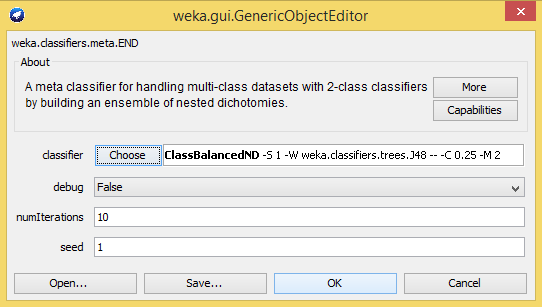
\includegraphics[width=9cm, height=5cm]{images/altera_end}}
	\caption {Alteração de classificador no algoritmo de meta-aprendizagem \textit{END}.}
	\label{end}
\end{figure}

Através das regras utilizadas pelo algoritmo, pode-se constatar que foram classificados corretamente como desligado:

\begin{itemize}
	\item 100\% dos alunos reprovados com menção TR ou TJ, 90,91\% com menção SR, 96,72\% com menção II e 74,36\% que obtiveram crédito concedido em Computação Básica;
	\item 61,75\% dos alunos reprovados com menção MI, 95,17\% com menção SR, 68,36\% com menção II e 95,16\% com menção TR em Física 3, dada a aprovação em Computação Básica com menção SS;
	\item 73,24\% dos alunos aprovados com menção MM em Computação Básica e Física 2 e reprovados com menção SR em Cálculo 3;
	\item  68,31\% dos alunos reprovados com menção MI, 95,15\% com menção II, 95,15\% com menção SR e 95,16\% com menção SR em Física 2, dada a aprovação em Computação Básica com menção MM;
	\item 66,26\% dos alunos reprovados com menção MI, 96,67\% com menção II e 96,54\% com menção SR em Física 2, dada a aprovação em Computação Básica com menção MS;
	\item 57,10\% dos alunos reprovados com menção MI, 100\% com menção SR e 73,82\% com menção II em Estruturas de Dados, dada a aprovação em Computação Básica e Física 2 com menção MS.
\end{itemize}

Analisando as taxas de classificação geradas pelos algoritmos conforme mostrado na Tabela \ref{cursando_geral}, foi possível identificar que entre os alunos que estavam cursando em 2014, 30\% a 54\% foram classificados como desligados, enquanto que 24\% a 31\% foram considerados formados, indicando que os alunos têm maior propensão a serem desligados do curso antes da conclusão. Considerando a taxa de desligamento, 30,06\% dos alunos irão desligar-se no melhor caso e 53,99\% no pior caso. Considerando a taxa de formatura, 30,67\% dos alunos irão formar-se no melhor caso e 24,54\% no pior caso. Para ambos os casos, o algoritmo \textit{DecisionTable} apresentou a maior taxa de predição para prováveis formados e desligados.

\begin{table} [!h]
	\centering
	\caption{Análise das matrizes de confusão dos algoritmos para os alunos identificados como cursando em 2014.} 
	\begin{tabular}{C{5cm}|C{3cm}C{3cm}C{3cm}}
		\hline
		\multicolumn{1}{c}{Algoritmo} & \multicolumn{3}{|c}{Percentual (\%) de classificação dos cursandos em 2014}\\ \hline
		& Formado & Desligado & Cursando\\
		\hline
		J48 &  24,54 & 30,06 & 45,40\\
		J48graft & 24,54 & 30,37 & 45,09 \\
		DecisionTable & 30,67 & 53,99 & 15,34 \\
		PART & 27,91 & 32,31 & 39,78 \\
		AttributteSelectedClassifier & 26,07 & 32,82 & 41,11\\
		END & 27,91 & 49,39 & 22,70\\	
		\hline
	\end{tabular}
	\label{cursando_geral}
\end{table}

A partir dos algoritmos de clusterização \textit{SimpleKMeans} e \textit{FatherstFirst}, foi realizada a análise dos \textit{clusters} gerados a partir dos atributos \textit{AluSexo} e \textit{AluSituacao}. Pelo algoritmo \textit{SimpleKMeans}, foram gerados dois \textit{clusters}, onde  63\% das instâncias pertencem ao \textit{cluster} 0 e o ponto centroide é representado pelos alunos do sexo masculino formados. Em 37\% das instâncias pertencem ao \textit{cluster} 1 e  o ponto centroide é representado pelos alunos do sexo masculino desligados, conforme mostrado na Figura \ref{cluster-kmeans}.

\begin{figure}[!h]
	\centering
	{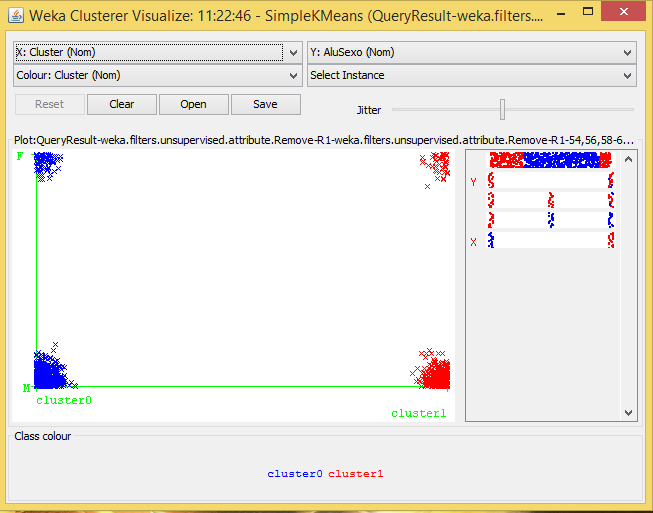
\includegraphics[width=10cm, height=8cm]{images/cluster-kmeans}}
	\caption {\textit{Cluster} gerado pelo algoritmo \textit{SimpleKmeans}, a partir dos atributos \textit{AluSexo} e \textit{AluSituacao}.}
	\label{cluster-kmeans}
\end{figure}
 
 O algoritmo \textit{FatherstFirst} também gerou dois \textit{clusters}, onde 41\% das instâncias pertencem ao \textit{cluster} 0, e o ponto centroide é representado pelos alunos do sexo feminino formado, e  59\% das instâncias pertencem ao \textit{cluster} 1 e o ponto centroide é representado pelos alunos do sexo masculino desligados, conforme mostrado na Figura \ref{cluster-first}.
 
 \begin{figure}[!h]
 	\centering
 	{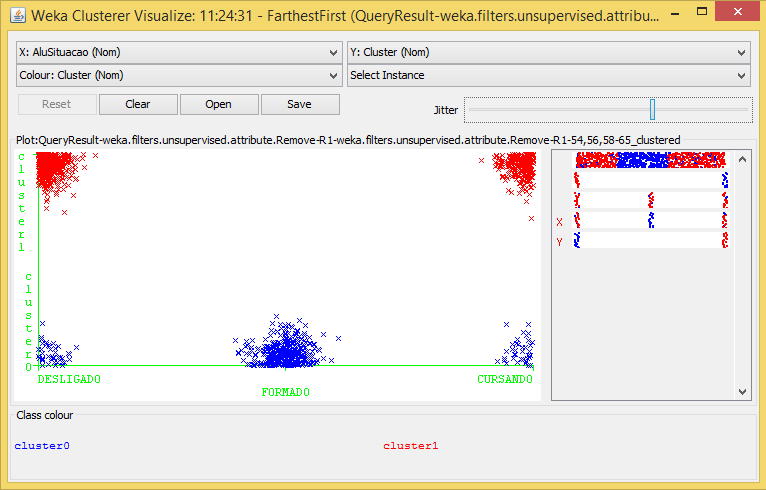
\includegraphics[width=10cm, height=8cm]{images/cluster-first}}
 	\caption {\textit{Cluster} gerado pelo algoritmo \textit{FatherstFisrt}, a partir dos atributos \textit{AluSexo} e \textit{AluSituacao}.}
 	\label{cluster-first}
 \end{figure}
 
\subsection{Evasão dos Alunos nos Semestres com Maiores Taxas de Desligamento} \label{resultado2}

Para a análise dos dados por semestre de ingresso, foram selecionados os algoritmos que apresentaram os melhores conjuntos de regras (que utilizaram maior número de atributos no conjunto de regras ou que apresentaram padrões precisos) e que apresentaram maiores taxas de acerto, considerando o número de instâncias que foram classificadas corretamente e a estatística \textit{Kappa} dos algoritmos, que mede a precisão de predição de uma classe verdadeira. A Estatística \textit{Kappa} varia entre 0 e 1, considerando que quanto mais próximo do valor 1 melhor o desempenho do algoritmo na classificação das instâncias. Pelo fato de cada algoritmo gerar uma regra específica para classificação, buscou-se comparar as regras e identificar similaridades nos padrões de regras utilizadas pelos algoritmos selecionados. 

\subsubsection{Ingressantes no Segundo Semestre de 2002}
Para o conjunto de dados do segundo semestre de 2002, os algoritmos que apresentaram as melhores regras e melhor desempenho foram os algoritmos de árvore \textit{ADTree, BFTree e LADTree}, o algoritmo de regras \textit{JRip} e os algoritmos de meta-aprendizagem \textit{Bagging, MultiBoostAB} e \textit{RandomCommitee}, conforme mostrado na Tabela \ref{algoritmos2_2002}.

\begin{table} [!h]
	\centering
	\caption{Algoritmos utilizados para os dados do segundo semestre de 2002.} 
	\begin{tabular}{C{3,5cm}|C{3,5cm}C{3,5cm}C{3,5cm}}
		\hline
		\multicolumn{1}{c}{Algoritmo} & \multicolumn{3}{|c}{Critérios de Avaliação}\\ \hline
		 & Instâncias Classificadas Corretamente (\%) & Instâncias Classificadas Incorretamente (\%) & Estatística \textit{Kappa}\\
		\hline
		ADTree &  85.7143 & 14.2857 & 0.7126\\
		BFTree & 88.5714 & 11.4286 & 0.7705\\
		LADTree & 94.2857 & 5.7143 & 0.8852\\
		JRip & 88.5714 & 11.4286 & 0.7697\\
		Bagging & 88.5714 & 11.4286 & 0.7697\\
		MultiBoostAB & 91.4286 & 8.5714 & 0.8276\\
		RandomCommitee & 88.5714 & 11.4286 &  0.7697\\
		
		\hline
	\end{tabular}
	\label{algoritmos2_2002}
\end{table}

Para o segundo semestre de 2002, uma das causas percebidas para justificar a evasão dos alunos foi a reprovação na disciplina de Computação Básica, dado que os algoritmos \textit{LADTree}, \textit{JRIP} e \textit{MultiBoostAB} classificaram os alunos que cursaram a disciplina Computação Básica mais de uma vez como desligados. Pelo algoritmo \textit{MultiBoostAB}, alunos que cursaram Computação Básica mais de uma vez foram identificados como desligados numa proporção de 100\%.

Uma exceção encontrada pelos algoritmos \textit{ADTree, BFTree}, \textit{LADTree}, e \textit{Bagging} e \textit{RandomCommitee} foi que os alunos que foram aprovados em Cálculo 2 pela primeira vez, com menção SS, foram identificados com desligados. Pelo algoritmo \textit{BFTree}, foram identificados três casos nesta condição no conjunto de teste gerado pelo algoritmo. Uma das possibilidades para justificar tal regra é o fato do conjunto de dados constituir uma amostra pequena.

Para o algoritmo \textit{ADTree}, as alunas foram classificados como desligadas. Para o algoritmo \textit{RandomCommitee}, os alunos que obtiveram SR como primeira menção em Física 3, MM como última menção em Programação Sistemática ou a última menção em Física 2 diferente de MM apresentaram maior probabilidade de serem classificados como desligados. O mesmo ocorre para a disciplina de Computação Básica, na qual alunos que obtiveram menção MI ao cursar a disciplina pela primeira vez foram classificados como desligados, conforme as regras geradas pelos algoritmos \textit{LADTree, Bagging, MultiBoostAB} e \textit{RandomComitee}, o que indica que o desempenho do  aluno na disciplina de Computação Básica foi um dos determinantes para o desligamento do aluno. 

Conforme a Tabela \ref{algoritmos2_2002}, o algoritmo de árvore de decisão \textit{LADTree} apresentou o melhor desempenho. A Figura \ref{ladtree2_2002} apresenta a regra de classificação utilizada pelo algoritmo, onde aproximadamente 94,3\% das instâncias foram classificadas corretamente.
 
 \begin{figure}[!h]
 	\centering
 	{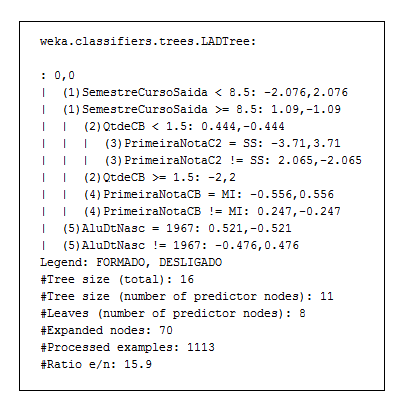
\includegraphics[width=8cm, height=8cm]{images/regra2_2002}}
 	\caption {Regra gerada pelo algoritmo de árvore \textit{LADTree}. Os valores positivos indicam se o aluno está formado ou desligado, conforme condição.}
 	\label{ladtree2_2002}
 \end{figure}
 
 
\subsubsection{Ingressantes no Primeiro Semestre de 2004}

Para o primeiro semestre de 2004, os algoritmos que apresentaram melhores desempenhos foram os algoritmos de árvore \textit{ADTree, J48graft} e \textit{LADTree}, o algoritmo de regras {OneR} e os algoritmos de meta-aprendizagem \textit{Bagging, MultiBoostAB} e \textit{RandomCommitee}, conforme apresentado na Tabela \ref{algoritmos1_2004}.

\begin{table} [!h]
	\centering
	\caption{ Algoritmos Utilizados para os dados do primeiro semestre de 2004.} 
	\begin{tabular}{C{3,5cm}|C{3,5cm}C{3,5cm}C{3,5cm}}
		\hline
		\multicolumn{1}{c}{Algoritmo} & \multicolumn{3}{|c}{Critérios de Avaliação}\\ \hline
		& Instâncias Classificadas Corretamente (\%) & Instâncias Classificadas Incorretamente (\%) & Estatística \textit{Kappa}\\
		\hline
		ADTree & 69.4444 & 30.5556 & 0.3125\\
		J48graft & 72.2222 & 27.7778 & 0.4156\\
		LADTree & 72.2222 & 27.7778 & 0.4156\\
		OneR & 66.6667 & 33.3333 & 0.3165\\
		Bagging &  77.7778 & 22.2222 & 0.5325\\
		MultiBoostAB & 75 & 25 & 0.4671\\
		RandomCommitee & 75 & 25 & 0.4527\\
		\hline
	\end{tabular}
	\label{algoritmos1_2004}
\end{table}

Todos os algoritmos apresentados na Tabela \ref{algoritmos1_2004} utilizaram atributos da disciplina Cálculo 3 em suas regras, em que alunos que foram aprovados em Cálculo 3 foram classificados como formados. Pela regra utilizada pelo algoritmo \textit{OneR}, os alunos que obtiveram menções MM e MS estão formados, e para as demais menções (II, TR, SR e SS) os alunos foram classificados como desligados. Em 88,89\% das instâncias foram classificadas corretamente neste caso.

Pelos algoritmos \textit{LADTree, Bagging } e \textit{MultiBoostAB}, os alunos que obtiveram MI como primeira menção na disciplina Estruturas de Dados foram classificados como desligados. Ainda para a disciplina Estruturas de Dados, o algoritmo \textit{J48graft} determinou que dada a aprovação do aluno em Cálculo 3, se o aluno cursou a disciplina mais de uma vez, este foi considerado desligados.

Para a disciplina Cálculo 2, foi verificado que os alunos que obtiveram MM como última nota foram classificados como desligados pelos algoritmos \textit{ADTree, LADTree} e \textit{MultiBoostAB}. Pelo algoritmo \textit{MultiBoostAB}, alunos que obtiveram MM como última menção em Cálculo 2 foram classificados em 89,95\% como desligados. 

Para a disciplina Programação Sistemática, os algoritmos \textit{ADTree, LADTree} e \textit{MultiBoostAB}, os alunos que obtiveram menção MS foram classificados como formados. Para as demais menções, o algoritmo \textit{MultiBoostAB} determinou em 77,88\% como desligados.

Para o primeiro semestre de 2004, a nota obtida em Cálculo 2 aparenta ser um dos fatores determinantes para a continuidade dos alunos ingressantes no semestre, o que pode indicar uma relação entre o desempenho do aluno em Cálculo 2 para Cálculo 3, visto que todos os algoritmos utilizaram a aprovação em Cálculo 3 como regra de classificação dos alunos. Outra justificativa é o fato de muitos alunos terem cursado Cálculo 3 nos semestres finais do curso, o que implica para os algoritmos que se o aluno não cursou Cálculo 3 ou obteve baixo desempenho, foram considerados desligados. Do mesmo modo, a aprovação na disciplina Estruturas de dados pode ser considerada um fator de decisão, já que os algoritmos também indicaram que alunos que cursaram Estruturas de Dados mais de uma vez foram classificados como desligados.  

Conforme a Tabela \ref{algoritmos1_2004}, o algoritmo que apresentou o melhor desempenho foi o algoritmo de regra \textit{Bagging}, onde aproximadamente 77,8\% das instâncias foram classificadas corretamente. Ao todo, foram geradas 10 árvores de decisão distintas pelo algoritmo. A Figura \ref{regra1_2004} apresenta uma delas como exemplo.

 \begin{figure}[!h]
 	\centering
 	{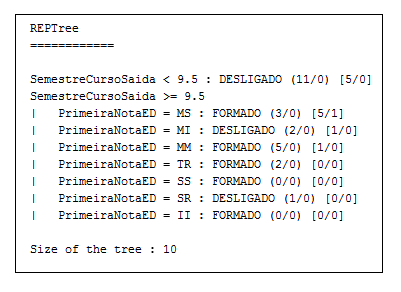
\includegraphics[width=9cm, height=6.5cm]{images/regra1_2004}}
 	\caption {Uma das regras geradas pelo algoritmo de regras \textit{Bagging} para os dados do primeiro semestre de 2004.}
 	\label{regra1_2004}
 \end{figure}

\subsubsection{Ingressantes no Segundo Semestre de 2005}

Para os dados do segundo semestre de 2005, foram utilizados os algoritmos de árvore \textit{ADTree, BFTree, LADTree} e \textit{SimpleCart}, e os algoritmos de meta-aprendizagem \textit{AdaBoostM1, MultiBoostAB} e \textit{RandomSubSpace}, conforme apresentado na Tabela \ref{algoritmos2_2005}. Os algoritmos de regras não foram considerados, por não apresentarem novas regras e padrões desconhecidos para o conjunto de dados.

\begin{table} [!h]
	\centering
	\caption{ Algoritmos Utilizados para os dados do segundo semestre de 2005.} 
	\begin{tabular}{C{3,5cm}|C{3,5cm}C{3,5cm}C{3,5cm}}
		\hline
		\multicolumn{1}{c}{Algoritmo} & \multicolumn{3}{|c}{Critérios de Avaliação}\\ \hline
		& Instâncias Classificadas Corretamente (\%) & Instâncias Classificadas Incorretamente (\%) & Estatística \textit{Kappa}\\
		\hline
		ADTree &  86.8421 & 13.1579 & 0.7383\\
		BFTree & 69.4444 & 30.5556 &  0.4\\
		LADTree & 72.2222 & 27.7778 &  0.4714\\
		SimpleCart & 69.4444 & 30.5556 & 0.489\\
		AdaBoostM1 & 72.2222 & 27.7778 & 0.4578\\
		MultiBoostAB & 75 & 25 & 0.5207\\
		RandomSubSpace & 72.2222 & 27.7778 & 0.4643\\
		\hline
	\end{tabular}
	\label{algoritmos2_2005}
\end{table}

Um padrão identificado, em todos os algoritmos, foi a utilização do atributo referente à ultima turma de Cálculo 2 nas regras de classificação. Em todas as regras geradas, foram classificados como formados os alunos que cursaram Cálculo 2 na turma K no primeiro semestre de 2006. Outro padrão identificado pelos algoritmos \textit{ADTree, LADTree, AdaBoostM1} e \textit{MultiBoostAB} é que alunos que obtiveram SR como primeira menção na disciplina Física 3 foram identificados como desligados. Todos os algoritmos de árvore de decisão classificaram como desligados os alunos que saíram antes do ano de 2007.

Pelo algoritmo \textit{LADTree} e \textit{AdaBoostM1}, foram classificados como formados os alunos que cursaram Física 2 na turma K no primeiro semestre de 2006. Pelos algoritmos \textit{ADTree, LADTree} e \textit{AdaBoostM1}, alunos que obtiveram a primeira menção em Estruturas de Dados diferente de MM foram considerados desligados. 

Para os dados deste semestre, as turmas nas quais foram cursadas as disciplinas de Cálculo 2 e o desempenho na disciplina Estruturas de Dados foram os fatores que mais influenciaram na continuidade dos alunos. Outra tendência percebida é que os alunos que obtêm SR ao cursar Física 3 pela primeira vez têm maior propensão a evadir do curso, o que pode indicar uma dificuldade por parte dos alunos para a disciplina. Ao analisar as turmas de Cálculo 2, percebe-se que vários fatores podem estar relacionados ao desempenho da turma, que podem estar relacionados ao conteúdo, ao docente (didática empregada, formas de avaliação, entre outros), ou ao aluno (motivação, tempo dedicado aos estudos, facilidade ou dificuldade de assimilação dos conteúdos), o que exige uma estudo mais detalhado e aprofundado.

Dos algoritmos utilizados, o que apresentou o melhor desempenho foi o \textit{ADTree}, pois aproximadamente 86,8\% das instâncias foram classificadas corretamente. A regra gerada é apresentada na Figura \ref{regra2_2005}. 

 \begin{figure}[!h]
 	\centering
 	{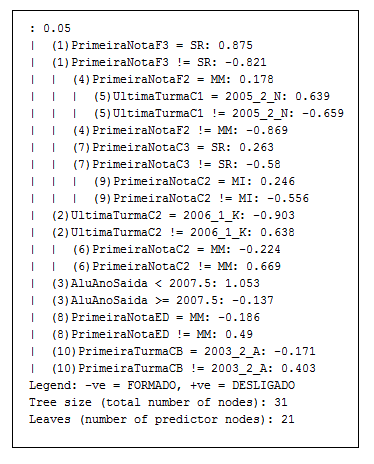
\includegraphics[width=11cm, height=11cm]{images/regra2_2005}}
 	\caption {Regra gerada pelo algoritmo de árvore de decisão \textit{ADTree} para os dados do segundo semestre de 2005.}
 	\label{regra2_2005}
 \end{figure}


\subsubsection{Ingressantes no Primeiro Semestre de 2006}

Para os dados do primeiro semestre de 2006, foram utilizados os algoritmos de árvore \textit{ADTree, BFTree, LADTree} e \textit{SimpleCart}, e os algoritmos de meta-aprendizagem \textit{Bagging, LogitBoost} e \textit{MultiBoostAB}, conforme apresentado na Tabela \ref{algoritmos1_2006}. Os algoritmos de regras não foram utilizados para a análise deste conjunto.

\begin{table} [!h]
	\centering
	\caption{ Algoritmos Utilizados para os dados do primeiro semestre de 2006.} 
	\begin{tabular}{C{3,5cm}|C{3,5cm}C{3,5cm}C{3,5cm}}
		\hline
		\multicolumn{1}{c}{Algoritmo} & \multicolumn{3}{|c}{Critérios de Avaliação}\\ \hline
		& Instâncias Classificadas Corretamente (\%) & Instâncias Classificadas Incorretamente (\%) & Estatística \textit{Kappa}\\
		\hline
		ADTree &  80 & 20 & 0.604\\
		BFTree & 82.5 & 17.5 &  0.6552\\
		LADTree & 85 & 15 & 0.703\\
		SimpleCart & 82.5 & 17.5 & 0.6552\\
		Bagging & 82.5 & 17.5 & 0.6517\\
		LogitBoost & 80 & 20 &  0.6\\
		MultiBoostAB & 82.5 & 17.5 & 0.6552\\
		\hline
	\end{tabular}
	\label{algoritmos1_2006}
\end{table}

Todos os algoritmos, com exceção dos algoritmos \textit{Bagging} e \textit{MultiBoostAB}, utilizaram atributos relacionados à disciplina Física 3 em suas regras de classificação. Pelos algoritmos de árvore de decisão, os alunos que cursaram Física 3 na turma D no segundo semestre de 2007 foram classificados como formados. Junto à disciplina de Física 3, a aprovação em Programação Sistemática foi utilizada pelos algoritmos \textit{ADTree, LogitBoost} e \textit{MultiBoostAB}, no qual alunos que obtiveram menção MS foram classificados como formados, e os alunos que obtiveram menções diferente de MS foram classificados como desligados. Pelo algoritmo \textit{MultiBoostAB}, alunos que obtiveram menção MS na disciplina Programação Sistemática foram classificados em 79,93\% dos casos como formados. Alunos que foram aprovados em Física 3 e Cálculo 3 foram classificados como aprovados.

Pela análise dos algoritmos e das regras geradas, percebe-se que a maior dificuldade dos alunos encontra-se nas disciplinas do terceiro semestre do curso, tais como Física 3 e Programação Sistemática, o que pode indicar que nesse grupo os alunos obtiveram um bom desempenho nos dois primeiros semestres.

O algoritmo \textit{LADTree} apresentou o melhor desempenho para os dados do primeiro semestre de 2006, pois 85\% das instâncias foram classificadas corretamente. A regra gerada pelo algoritmo é mostrada na Figura \ref{regra1_2006}. 


 \begin{figure}[!h]
 	\centering
 	{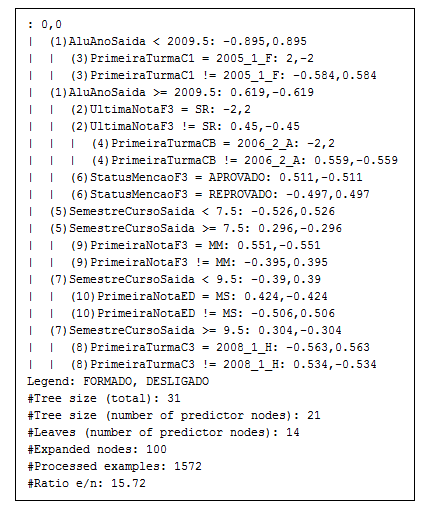
\includegraphics[width=10cm, height=12cm]{images/regra1_2006}}
 	\caption {Regra gerada pelo algoritmo de árvore \textit{LADTree} para os dados do primeiro semestre de 2006.}
 	\label{regra1_2006}
 \end{figure}

\subsubsection{Ingressantes no Segundo Semestre de 2006}

Para os dados do segundo semestre de 2006, foram utilizados os algoritmos de árvore \textit{BFTree, J48, J48graft} e \textit{LADTree}, o algoritmo de regra \textit{Ridor} e os algoritmos de meta-aprendizagem \textit{FilteredClassifier} e \textit{RandomCommittee}, conforme apresentado na Tabela \ref{algoritmos2_2006}.

\begin{table} [!h]
	\centering
	\caption{ Algoritmos Utilizados para os dados do segundo semestre de 2006.} 
	\begin{tabular}{C{3,5cm}|C{3,5cm}C{3,5cm}C{3,5cm}}
		\hline
		\multicolumn{1}{c}{Algoritmo} & \multicolumn{3}{|c}{Critérios de Avaliação}\\ \hline
		& Instâncias Classificadas Corretamente (\%) & Instâncias Classificadas Incorretamente (\%) & Estatística \textit{Kappa}\\
		\hline
		BFTree &  86.1111 & 13.8889 & 0.7309\\
		J48 & 83.3333 & 16.6667 &  0.6776\\
		J48graft & 83.3333 & 16.6667 &  0.6776\\
		LADTree & 86.1111 & 13.8889 & 0.7293\\
		Ridor & 86.1111 & 13.8889 & 0.7309\\
		FilteredClassifier & 86.1111 & 13.8889 &   0.7309\\
		RandomCommittee & 83.3333 & 16.6667 & 0.6766\\
		\hline
	\end{tabular}
	\label{algoritmos2_2006}
\end{table}

Os algoritmos \textit{BFTree, J48, FilterClassifier} e \textit{RandomCommitee} utilizaram a primeira turma da disciplina Estruturas de Dados para classificar os alunos como formados ou desligados, porém os algoritmos \textit{BFTree} e \textit{FilteredClassifier} apresentaram melhores desempenhos, ambos classificando aproximadamente 86,1\% das instâncias corretamente. Comparando as duas regras geradas, os alunos que cursaram Estruturas de Dados pela primeira vez na turma E no primeiro semestre de 2010, na turma A no primeiro semestre de 2008 ou na turma C no segundo semestre de 2004 foram classificados como desligados, dado que o aluno saiu do curso depois do ano de 2009. Pelo algoritmo \textit{J48graft}, o aluno que cursou Estruturas de Dados na turma C no segundo semestre de 2004 foi classificado como desligado dado que o aluno não tenha cursado Física 1 na turma A no segundo semestre de 2006.

Pelos algoritmos \textit{J48graft} e \textit{LADTree}, os alunos que cursaram Física 1 na turma A no segundo semestre de 2006 foram classificados como formados, da mesma forma que os alunos que cursaram Cálculo 2 na turma K no primeiro semestre de 2007 e os alunos que cursaram Física 1 na turma A no segundo semestre de 2006. Pelos algoritmos \textit{LADTree} e \textit{RandomCommittee}, alunos que foram aprovados em Cálculo 1 ao cursar a disciplina pela primeira vez foram classificados como aprovados.

Analisando as regras apresentadas, percebe-se que os atributos relacionados à disciplina Estruturas de Dados foram utilizados pela maioria dos algoritmos, o que indica que a turma na qual o aluno cursou a disciplina pela primeira vez pode estar influenciando no desempenho posterior do aluno, seja de forma direta ou indireta.

Entre os algoritmos utilizados, o \textit{BFTree, Ridor} e \textit{FilteredClassifier} apresentaram melhores desempenhos, ambos identificado aproximadamente 86,1\% das instâncias classificadas corretamente. A Figura \ref{regra2_2006} apresenta a regra de classificação gerada pelo algoritmo \textit{FilteredClassifier}. Os números entre parênteses representam, respectivamente, o número de instâncias abrangidas pela regra e o número de instâncias classificadas incorretamente, ambos separados por uma barra.

 \begin{figure}[!h]
 	\centering
 	{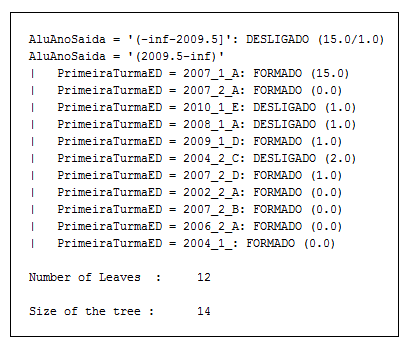
\includegraphics[width=11cm, height=10cm]{images/regra2_2006}}
 	\caption {Regra gerada pelo algoritmo de meta-aprendizagem \textit{FilteredClassifier} para os dados do segundo semestre de 2006.}
 	\label{regra2_2006}
 \end{figure}


\subsubsection{Ingressantes no Segundo Semestre de 2009}

Para os dados do segundo semestre de 2009, foram utilizados o algoritmo de árvore \textit{J48graft}, o algoritmo de regras \textit{JRip} e os algoritmos de meta-aprendizagem \textit{AdaBoostM1, Bagging, Decorate} e \textit{LogitBoost}, conforme apresentado na Tabela \ref{algoritmos2_2009}.

\begin{table} [!h]
	\centering
	\caption{ Algoritmos Utilizados para os dados do segundo semestre de 2006.} 
	\begin{tabular}{C{3,5cm}|C{3,5cm}C{3,5cm}C{3,5cm}}
		\hline
		\multicolumn{1}{c}{Algoritmo} & \multicolumn{3}{|c}{Critérios de Avaliação}\\ \hline
		& Instâncias Classificadas Corretamente (\%) & Instâncias Classificadas Incorretamente (\%) & Estatística \textit{Kappa}\\
		\hline
		J48graft &  93.75 & 6.25 & 0.8822\\
		JRip &  97.9167 & 2.0833 &  0.962\\
		AdaBoostM1 & 89.5833 & 10.4167 & 0.8098\\
		Bagging & 93.75 & 6.25 & 0.8822\\
		Decorate & 93.75 & 6.25 & 0.8822\\
		LogitBoost & 91.6667 & 8.3333 & 0.8502\\
		\hline
	\end{tabular}
	\label{algoritmos2_2009}
\end{table}

Os algoritmos \textit{J48graft, Bagging} e \textit{LogitBoost} identificaram os alunos que foram aprovados com menção MM em Física 1 como desligados. Pelo algoritmo \textit{AdaBoost}, alunos aprovados com menção MM em Física 1 foram classificados em 57,61\% como desligados. Outro padrão identificado pelos algoritmos é que alunos que cursaram a disciplina Programação Sistemática na turma A no segundo semestre de 2010 foram classificados como formados.

Por meio das regras apresentadas, o desempenho na disciplina de Física 1 pode ser considerada um fator determinante no processo de evasão, visto que por ser uma disciplina inicial, a não aprovação nesta disciplina ou um baixo rendimento, mesmo o aluno sendo aprovado, poderá impactar nas disciplinas subsequentes.

O algoritmo que apresentou o melhor desempenho para os dados do segundo semestre de 2009 foi o \textit{JRip}, onde aproximadamente 97,9\% das instâncias foram classificadas corretamente. A Figura \ref{regra2_2009} apresenta a regra de classificação utilizada pelo algoritmo.

 \begin{figure}[!h]
 	\centering
 	{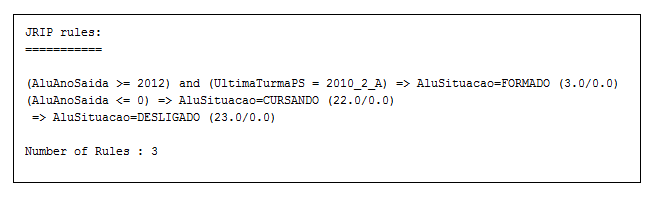
\includegraphics[width=11cm, height=4cm]{images/regra2_2009}}
 	\caption {Regra gerada pelo algoritmo de regras \textit{JRip} para os dados do segundo semestre de 2009.}
 	\label{regra2_2009}
 \end{figure}

\subsubsection{Ingressantes no Segundo Semestre de 2011}

Para os dados do segundo semestre de 2011, foram utilizados o algoritmo de árvore \textit{LADTree}, o algoritmo de regra \textit{JRip} e os algoritmos de meta-aprendizagem \textit{Bagging, FilteredClassifier, MultiBoostAB, OrdinalClassClassifier} e \textit{RandomSubSpace}, conforme apresentado na Tabela \ref{algoritmos2_2011}.


\begin{table} [!h]
	\centering
	\caption{ Algoritmos Utilizados para os dados do segundo semestre de 2011.} 
	\begin{tabular}{C{3,5cm}|C{3,5cm}C{3,5cm}C{3,5cm}}
		\hline
		\multicolumn{1}{c}{Algoritmo} & \multicolumn{3}{|c}{Critérios de Avaliação}\\ \hline
		& Instâncias Classificadas Corretamente (\%) & Instâncias Classificadas Incorretamente (\%) & Estatística \textit{Kappa}\\
		\hline
		LADTree & 80.4348 & 19.5652 & 0.6057\\
		JRip & 86.9565 & 13.0435 & 0.7386\\
		Bagging & 82.6087 & 17.3913 & 0.6515\\
		FilteredClassifier & 86.9565 & 13.0435 & 0.7386\\
		MultiBoostAB & 82.6087 & 17.3913 & 0.6515\\
		OrdinalClassClassifier & 86.9565 & 13.0435 & 0.7386\\
		RandomSubSpace & 82.6087 & 17.3913 & 0.6515\\
		\hline
	\end{tabular}
	\label{algoritmos2_2011}
\end{table}

Todos os algoritmos utilizaram a disciplina Física 1 como ponto de análise inicial. Através dos algoritmos \textit{Bagging} e \textit{RandomSubSpace}, os alunos com menções MI, II e SR em Física 1 foram classificados como desligados. Dado que o aluno foi aprovado em Física 1, a aprovação em Programação Sistemática foi determinante para classificar se o aluno está cursando ou desligado. Pelos algoritmos \textit{LADTree} e \textit{MultiBoostAB}, alunos que obtiveram SR em Programação Sistemática foram classificados como desligados.

Analisando os padrões detectados pelos algoritmos, as disciplinas de Física 1 e Programação Sistemática foram determinantes para os algoritmos classificarem o aluno como cursando ou desligado. Dado que todos os algoritmos identificaram Física 1 como origem das regras, percebe-se que os alunos ingressantes nesse semestre encontraram dificuldades na disciplina.

Os algoritmos que apresentaram os melhores desempenhos foram  \textit{JRip, FilteredClassifier} e o \textit{OrdinalClassClassifier}, pois ambos classificaram aproximadamente 87\% das instâncias corretamente. Analisando as matrizes de confusão dos algoritmos, 3 alunos cursando foram identificados como desligados e 3 alunos desligados foram identificados como cursando. A Figura \ref{regra2_2011} apresenta a regra de classificação utilizada pelo algoritmo \textit{JRip}. 

 \begin{figure}[!h]
 	\centering
 	{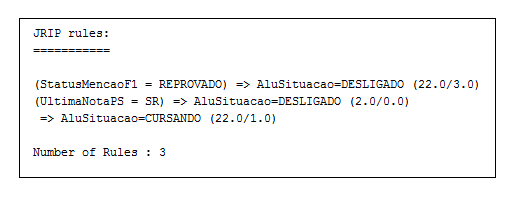
\includegraphics[width=11cm, height=4cm]{images/regra2_2011}}
 	\caption {Regra gerada pelo algoritmo de regras \textit{JRip} para os dados do segundo semestre de 2011.}
 	\label{regra2_2011}
 \end{figure}